\documentclass[11pt,a4paper]{article}
\usepackage[utf8]{inputenc}
\usepackage[T1]{fontenc}
\usepackage[spanish,es-nodecimaldot]{babel}
\usepackage{lmodern}
\usepackage{geometry,booktabs,tabularx,array,enumitem,amsmath,graphicx,float,caption,hyperref}
\geometry{top=2.3cm,bottom=2.3cm,left=2.4cm,right=2.4cm}
\hypersetup{colorlinks=true,linkcolor=black,urlcolor=blue}
\setlength{\parindent}{0pt}
\setlength{\parskip}{0.55em}
\setlength{\tabcolsep}{4pt}
\renewcommand{\arraystretch}{1.15}
\setlist{leftmargin=*,topsep=3pt,itemsep=3pt}
\newcolumntype{Y}{>{\raggedright\arraybackslash}X}
\emergencystretch=2em
\raggedbottom

\title{\textbf{Exploración de modelos de inteligencia artificial multimodal\\
para la identificación de macromicetos mediante dispositivos móviles}\\[0.6em]
\normalsize Resultados de las semanas 7 y 8: recortes de imagen e integración ambiental}
\author{Daniel Esteban Camacho Ospina\\Cesar Augusto Pulido Cuervo}
\date{}

\begin{document}
\maketitle

\begin{abstract}
Se presenta el estudio de recortes geométricos de imágenes y la primera
integración de información ambiental con un clasificador visual de
macromicetos. Los ensayos se realizaron sobre la versión \texttt{v002} de
FungiTastic y se compararon en la partición oficial de validación. En la
comparación controlada de recortes, ambos modelos se evaluaron con el mismo
recorte central: el control obtuvo un F1 macro por observación de 0,9738 y el
modelo entrenado con recortes alcanzó 0,9770. La diferencia no demostró una
ventaja concluyente de esta modificación. Para multimodalidad se
entrenaron tres variantes: visual, ambiental y combinada. La primera y la
tercera alcanzaron 0,9771 en validación, mientras que la ambiental obtuvo
0,1890. La fusión ensayada no mostró una mejora en la decisión por observación.
Los resultados describen las condiciones evaluadas y no constituyen una
evaluación final en test.
\end{abstract}

\section{Objetivo y alcance}
La semana 7 se dedicó a estudiar el efecto de modificar el encuadre de las
fotografías, tanto en las predicciones como en el ajuste de los parámetros del
modelo. En este trabajo, \emph{segmentación} se refiere a recortes geométricos
de la imagen; no se entrenó un modelo de segmentación por píxel ni se generaron
máscaras del hongo.

La semana 8 se enfocó en diseñar y evaluar una primera fusión entre información
visual y metadatos ambientales. Se contrastaron un modelo solo visual, uno
solo ambiental y otro que combina ambas modalidades, bajo una configuración
común de entrenamiento y validación.

\section{Datos y protocolo experimental}
Se utilizó exclusivamente FungiTastic \texttt{v002}, con diez géneros y las
particiones oficiales. La tabla~\ref{tab:particiones} resume su composición.
Las imágenes de una misma observación permanecen en la partición asignada a
esa observación. Durante estas campañas se utilizaron únicamente entrenamiento
y validación; no se ejecutó una nueva evaluación en test.

\begin{table}[H]
\centering
\caption{Composición de las particiones oficiales de \texttt{v002}.}
\label{tab:particiones}
\begin{tabular}{lrrl}
\toprule
Partición & Observaciones & Imágenes & Función \\
\midrule
Train & 17\,799 & 30\,172 & Ajuste de parámetros \\
Validación & 3\,452 & 6\,290 & Selección y comparación \\
Test & 4\,039 & 7\,159 & Evaluación final reservada \\
\bottomrule
\end{tabular}
\end{table}

La unidad principal de evaluación es la observación. Si un registro tiene
varias fotografías, las probabilidades producidas para cada una se promedian y
se selecciona el género con mayor probabilidad media. La métrica principal es el
\textbf{F1 macro por observación}: calcula el F1 de cada género y promedia los
diez valores con igual peso. Esta métrica complementa la exactitud, que puede
estar dominada por los géneros más frecuentes.

Las comparaciones de estas semanas se realizaron en validación, utilizada
también para elegir el mejor checkpoint. Por tanto, no representan una medición
independiente del proceso de selección. Además, test había sido consultado
históricamente para ResNet-18 en una fase anterior del proyecto; esa exposición
debe considerarse al interpretar cualquier evaluación posterior.

\section{Semana 7: estudio de recortes}
\subsection{Diseño}
Se partió del checkpoint visual de MobileNetV3-Large seleccionado en el ensayo
C. En este experimento, \textbf{entrenamiento control} significa continuar el
ajuste del modelo con las fotografías en su encuadre habitual, sin añadir el
recorte central estudiado. \textbf{Entrenamiento con recorte} significa
continuar el ajuste usando esas mismas fotografías después de aplicar un
recorte central que conserva el 75\,\% del área original; luego se aplican las
transformaciones habituales. Por tanto, se comparan dos modelos que parten del
mismo checkpoint y difieren en el encuadre que reciben durante el ajuste.
Ambos conservan los aumentos habituales, incluido el recorte aleatorio de
entrenamiento; «control» indica que no se añade el recorte central fijo del
75\,\%. Durante la evaluación, «original» indica el procesamiento habitual
de redimensionamiento y recorte a la entrada del modelo, sin ese recorte
adicional del 75\,\%.

Después, cada modelo se evaluó con ambos encuadres: la fotografía original y
el recorte central del 75\,\% del área. Por ejemplo, la fila «Control / recorte
75\,\%» corresponde al modelo entrenado con fotografías originales, al que se
le presentan recortes durante la evaluación. Este cruce permite separar el
efecto del encuadre de evaluación del efecto de haber entrenado con recortes.
El 75\,\% se refiere al área conservada, no al ancho ni a la altura. El recorte
es geométrico y no garantiza que la región retenida corresponda al hongo.
Ambas continuaciones usaron un máximo de diez épocas y parada temprana;
terminaron en la época 4 y conservaron la época 1 como mejor resultado.

\subsection{Resultados de validación}
\begin{table}[H]
\centering
\caption{Comparación entre entrenamiento e inferencia con recorte.}
\label{tab:recortes}
\begin{tabular}{llrr}
\toprule
Entrenamiento & Encuadre de evaluación & F1 macro obs. & F1 macro imagen \\
\midrule
Control & Original & 0,9773 & 0,9332 \\
Control & Recorte central del 75\,\% & 0,9738 & 0,9350 \\
Con recorte & Original & 0,9661 & 0,9200 \\
Con recorte & Recorte central del 75\,\% & 0,9770 & 0,9346 \\
\bottomrule
\end{tabular}
\end{table}

La comparación directa del efecto de entrenar con recortes mantiene fijo el
encuadre de evaluación. Con el recorte en evaluación, la diferencia entre el
modelo entrenado con recortes y el control fue de $+0{,}0032$ en F1 macro por observación, con un
intervalo pareado del 95\,\% de $[-0{,}0010;\,0{,}0077]$. Con el encuadre
original la diferencia fue $-0{,}0112$, con intervalo
$[-0{,}0270;\,-0{,}0009]$. Los intervalos se obtuvieron mediante 10\,000
remuestreos pareados por observación; no incorporan la variación entre semillas
ni agrupan por sitio y día.

En las condiciones estudiadas, el recorte no mostró una ventaja concluyente al
comparar ambos modelos con el mismo encuadre recortado. Además, el modelo
ajustado con recortes rindió menos con el encuadre original. Esto sugiere que
la correspondencia entre el procesamiento de entrenamiento y el de uso merece
atención; no implica que todos los métodos de recorte sean perjudiciales.

\begin{figure}[H]
\centering
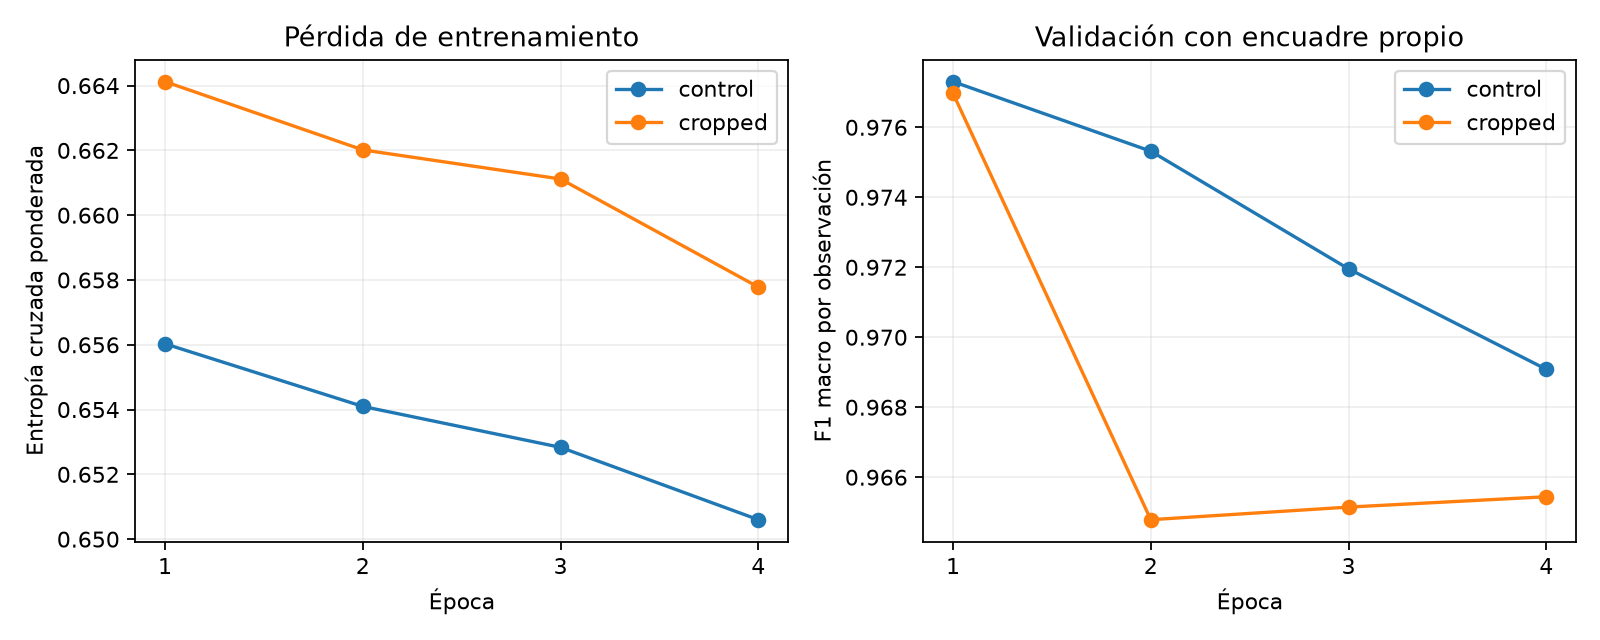
\includegraphics[width=0.86\linewidth]{images/training_curves.png}
\caption{Evolución de las continuaciones de control y con recortes. En la
curva de validación, el control recibe el encuadre original y el modelo con
recortes recibe el recorte central del 75\,\%.}
\end{figure}

\subsection{Estabilidad y parámetros}
Para estimar la variación del ajuste visual se repitió el control con tres
semillas, siempre desde el mismo checkpoint C y con el encuadre original.
Los resultados se resumen en la tabla~\ref{tab:semillas}.

\begin{table}[H]
\centering
\caption{Repeticiones del ajuste visual de control.}
\label{tab:semillas}
\begin{tabular}{rrrr}
\toprule
Semilla & Épocas ejecutadas & Mejor época & F1 macro obs. \\
\midrule
42 & 4 & 1 & 0,9773 \\
43 & 5 & 2 & 0,9700 \\
44 & 9 & 6 & 0,9723 \\
\bottomrule
\end{tabular}
\end{table}

La media fue 0,9732, con desviación estándar muestral de 0,0037. El checkpoint
C de partida registró 0,9717 en la misma validación. Los intervalos pareados de
las diferencias frente a C incluyeron cero en las tres repeticiones; por ello,
la mejora observada en una semilla no se considera demostrada de forma
consistente. Estas repeticiones miden la variación del ajuste posterior
condicionada al mismo checkpoint inicial, no la variabilidad de todo el
entrenamiento desde cero.

Se registraron las diferencias entre pesos del checkpoint inicial y de las
continuaciones. Una mayor variación de parámetros no implica por sí misma un
mejor clasificador. También se encontraron 40 observaciones con errores en las
tres semillas y 67 con predicciones diferentes entre ellas. Los géneros con
pocas observaciones requieren especial cuidado: \emph{Morchella} tiene 11
observaciones en validación, \emph{Hericium} 66 y \emph{Geastrum} 79.

\section{Semana 8: primera integración multimodal}
\subsection{Variables ambientales}
Se estudiaron hábitat, sustrato, elevación y fecha del registro. La
tabla~\ref{tab:ambiental} resume la disponibilidad de los campos auditados.
Todas las observaciones de train y validación tenían fecha disponible.
La información climática estaba ausente y, por tanto, no se incluyó.

\begin{table}[H]
\centering
\caption{Disponibilidad de metadatos en observaciones de train y validación.}
\label{tab:ambiental}
\begin{tabular}{lrr}
\toprule
Campo & Train & Validación \\
\midrule
Hábitat presente & 17\,799 & 3\,452 \\
Sustrato presente & 17\,799 & 3\,452 \\
Elevación con calidad aceptada & 10\,996 & 2\,197 \\
Datos climáticos ausentes & 17\,799 & 3\,452 \\
\bottomrule
\end{tabular}
\end{table}

El sustrato presenta baja precisión en 1\,811 observaciones de entrenamiento y
en una de validación. Esta diferencia requiere revisión, pues las particiones
pueden tener distintas condiciones de calidad. Parte de los metadatos procede
de anotaciones o de transformaciones de la fuente; su disponibilidad durante el
uso real y su relación con el proceso de identificación deben verificarse.

\subsection{Codificación y arquitectura}
Las categorías de hábitat y sustrato se codificaron a partir de los valores
observados en train, con una categoría para valores desconocidos o ausentes.
La elevación de calidad aceptada se estandarizó con la media y desviación de
train; los valores ausentes o no aceptados se acompañaron de un indicador.
La fecha se representó mediante dos componentes cíclicas del día del año y una
marca de ausencia o calidad no aceptada. No se usaron coordenadas, taxonomía,
identificadores, año ni variables climáticas como entradas del modelo.

El codificador se ajustó solo con observaciones de train y su estado se guardó
junto con los checkpoints. La unión entre imágenes y metadatos comprobó que
identificador, partición y etiqueta fueran consistentes. El entrenamiento usó
las imágenes como unidad, por lo que una observación con varias fotografías
contribuyó varias veces a la pérdida.

Se prepararon tres variantes:
\begin{itemize}
\item \textbf{Visual:} MobileNetV3-Large inicializado desde el checkpoint C y
ajustado con imágenes.
\item \textbf{Ambiental:} una capa lineal que recibe únicamente los metadatos
codificados.
\item \textbf{Multimodal:} MobileNetV3-Large inicializado desde el mismo
checkpoint C y una capa ambiental lineal cuyos resultados se suman a los
\emph{logits} visuales.
\end{itemize}

La capa ambiental del modelo multimodal se inicializó en cero, de modo que al
inicio reproduce las predicciones del modelo visual. La fusión aditiva es una
primera aproximación sencilla; no modela interacciones complejas entre las
características visuales y ambientales.

\subsection{Entrenamiento y resultados}
Las tres corridas utilizaron semilla 42, optimizador AdamW, tasa de aprendizaje
inicial de $10^{-4}$, ponderación de clases inversa a la raíz de su frecuencia,
hasta diez épocas y paciencia de tres épocas para parada temprana. La selección
del mejor checkpoint se realizó por F1 macro de observación en validación.
Los modos visual y multimodal terminaron en la época 4 con mejor época 1; el
ambiental terminó en la época 9 con mejor época 6.
El control visual de S8 es una nueva corrida para comparar las modalidades;
no debe confundirse con la corrida de control de S7.

\begin{table}[H]
\centering
\caption{Resultados de las tres variantes en validación normal.}
\label{tab:s8}
\begin{tabular}{lrrrr}
\toprule
Modalidad & Épocas & Mejor época & F1 macro obs. & Exactitud obs. \\
\midrule
Visual & 4 & 1 & 0,9771 & 0,9800 \\
Ambiental & 9 & 6 & 0,1890 & 0,4276 \\
Multimodal & 4 & 1 & 0,9771 & 0,9800 \\
\bottomrule
\end{tabular}
\end{table}

En esta primera prueba, el modelo basado solo en metadatos fue claramente
inferior al visual. La fusión no cambió las clases predichas para las
3\,452 observaciones frente al control visual, aunque sí se observaron
diferencias en probabilidades y en dos decisiones por imagen. Por ello,
la coincidencia en F1 no debe interpretarse como identidad de los modelos ni
como prueba de que los metadatos no puedan aportar en otras configuraciones.

\subsection{Sensibilidad a la información ambiental}
Se evaluaron los modelos ambiental y multimodal bajo dos perturbaciones:
ausencia de todos los campos ambientales y sustitución de metadatos entre
observaciones. La asignación intercambiada fue reproducible y conservó el
mismo conjunto de imágenes. Son escenarios controlados para estudiar
sensibilidad, no una representación directa de las condiciones de uso.

\begin{table}[H]
\centering
\caption{F1 macro por observación ante perturbaciones de metadatos.}
\label{tab:sensibilidad}
\begin{tabular}{lrrr}
\toprule
Modelo & Datos originales & Ausentes & Intercambiados \\
\midrule
Ambiental & 0,1890 & 0,0415 & 0,0796 \\
Multimodal & 0,9771 & 0,9771 & 0,9771 \\
\bottomrule
\end{tabular}
\end{table}

El modelo ambiental depende de la información recibida, mientras que la
decisión por observación del modelo multimodal permaneció igual en estas
condiciones. Frente a su evaluación normal, quitar los metadatos cambió una
decisión por imagen e intercambiarlos cambió dos, sin modificar las decisiones
agregadas por observación. Esto describe la fusión y el checkpoint seleccionados en este
ensayo. No demuestra invariancia de las probabilidades ni permite concluir
que el sistema sea robusto ante todas las alteraciones posibles.

\section{Conclusiones y trabajo siguiente}
Los experimentos de recortes no aportaron evidencia concluyente para sustituir
el procesamiento visual de referencia. La comparación con tres semillas
mostró variación del ajuste posterior y confirma la necesidad de interpretar
las diferencias pequeñas con cautela.

La primera fusión ambiental no mejoró el F1 macro por observación frente al
control visual y mantuvo las mismas decisiones por observación bajo las
perturbaciones examinadas. El clasificador solo ambiental ensayado obtuvo una
puntuación reducida. Esta comparación utiliza una semilla y una configuración
común; no demuestra el rendimiento máximo que podría alcanzar cada modalidad.

El trabajo siguiente comprende:
\begin{enumerate}
\item Revisar las observaciones con errores persistentes y el soporte reducido
de algunos géneros, sin modificar las particiones oficiales de \texttt{v002}.
\item Investigar la procedencia y diferencia de calidad del sustrato entre
train y validación, así como la disponibilidad real de cada campo en Android.
\item Estudiar la contribución de cada variable y repetir los experimentos
con varias semillas antes de atribuir mejoras a la fusión.
\item Evaluar alternativas de fusión y manejo de metadatos ausentes, manteniendo
el control visual y las mismas observaciones para una comparación justa.
\item Definir el protocolo de selección antes de cualquier evaluación final en
test y medir el desempeño y la latencia de la solución integrada en Android.
\end{enumerate}
\end{document}
